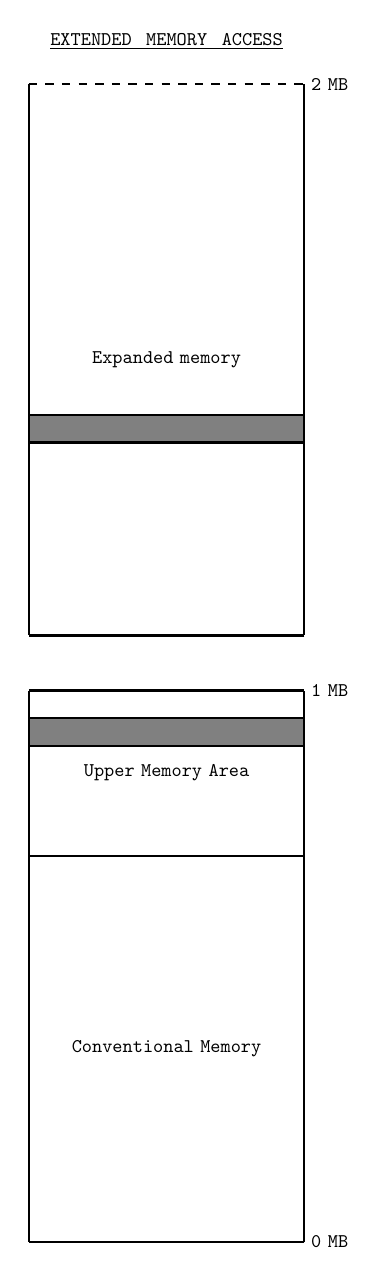
\begin{tikzpicture}[scale=0.7, every node/.style={scale=0.7}]


%Title
\node[above] at (2.5,21.5){$\mathtt{\Huge{\underline{EXTENDED\ MEMORY\ ACCESS}}}$}  ;

%Draw borders of ALL RAM
\draw[thick,black] (5,0)  -- (0,0);
\draw[thick,black] (5,0 ) -- (5,10);
\draw[thick,black] (0,10) -- (5,10);
\draw[thick,black] (0,10)  -- (0,0);

%Defining grey color
\colorlet{LighterMark}{black!50}

\node[right,align=left] at (5,0){$\mathtt{0\ MB}$}  ;

%UMA
\draw[thick,black] (0,7)  -- (5,7);

%Top RAM
\node[right,align=left] at (5,10){$\mathtt{1\ MB}$}  ;

\draw[thick,black] (5,11)  -- (0,11);
\draw[thick,black] (5,11 ) -- (5,21);
\draw[thick,black,dashed] (0,21) -- (5,21);
\draw[thick,black] (0,21)  -- (0,11);
\node[right,align=left] at (5,21){$\mathtt{2\ MB}$}  ;

\draw [thick,fill=LighterMark] (0,9) rectangle (5,9.5);
\draw [thick,fill=LighterMark] (0,14.5) rectangle (5,15);

\node[] at (2.5,3.5){$\mathtt{Conventional\ Memory}$}  ;
\node[] at (2.5,16){$\mathtt{Expanded\ memory}$}  ;
\node[] at (2.5,8.5){$\mathtt{Upper\ Memory\ Area}$}  ;

\end{tikzpicture}
